% generated by scripts/pkl_to_latex.py
% source PKL : uscan_v1_L8_Ne8_t0p1_mode-uniform_nmin2_solver-gcg_full_es_restarts10_iter300_kmax5_tol1em09_U0.1to5_N21-8081b758e7cc.pkl
% scan type  : uscan
% state      : ex_singlet
% quantity   : purity
% requires   : \usepackage{pgfplots} \pgfplotsset{compat=1.18}
% colours match the matplotlib PDF (tab10 cycle)
\definecolor{gmeC0}{HTML}{1F77B4}
\definecolor{gmeC1}{HTML}{FF7F0E}
\definecolor{gmeC2}{HTML}{2CA02C}
\definecolor{gmeC3}{HTML}{D62728}
\definecolor{gmeC4}{HTML}{9467BD}
\definecolor{gmeC5}{HTML}{8C564B}
\definecolor{gmeC6}{HTML}{E377C2}
\definecolor{gmeC7}{HTML}{17BECF}

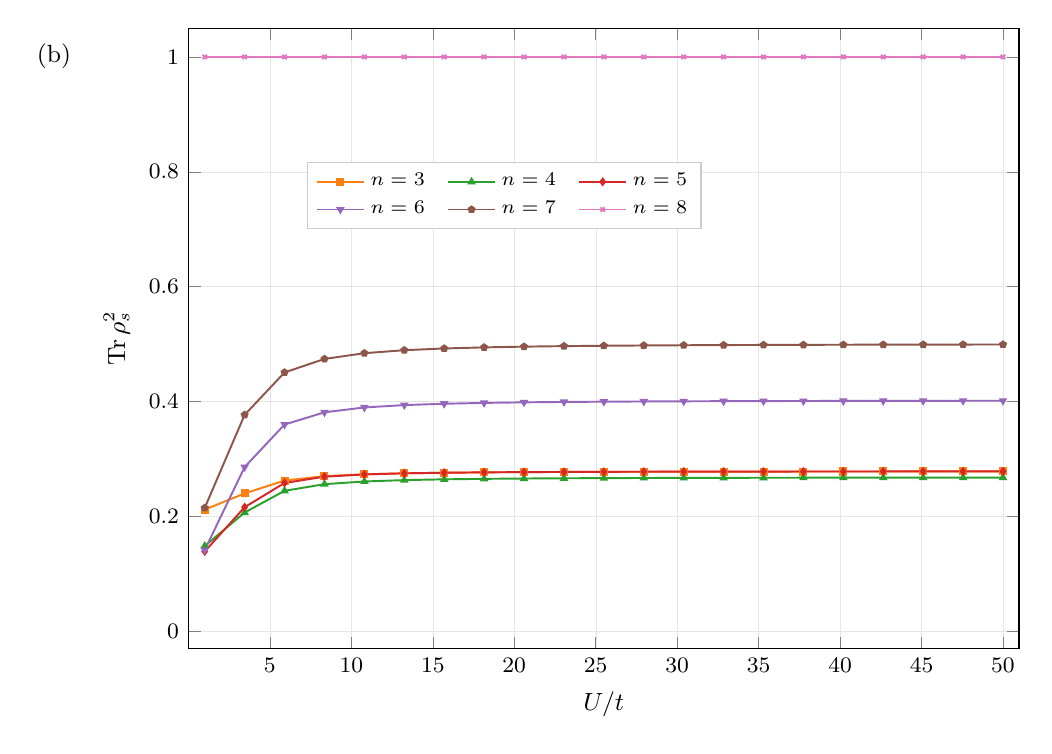
\begin{tikzpicture}
  \begin{axis}[
    width=\columnwidth,
    height=0.78\columnwidth,
    xlabel={$U/t$},
    ylabel={$\mathrm{Tr}\,\rho_s^2$},
    grid=both,
    grid style={line width=.1pt, draw=gray!20},
    tick label style={font=\footnotesize\rmfamily, /pgf/number format/fixed},
    label style={font=\small\rmfamily},
    scaled ticks=false,
    legend style={font=\scriptsize\rmfamily, draw=gray!40, at={(0.5,1.03)}, anchor=south, /tikz/every even column/.append style={column sep=6pt}},
    legend cell align={left},
    legend columns=3,
    ymin=-0.03,
    ymax=1.05,
    xmin=0.02,
    xmax=50.98,
    legend style={at={(0.380,0.730)}, anchor=center, fill=white},
    after end axis/.append code={\node[anchor=east, font=\small\rmfamily] at (axis description cs:-0.13,0.954) {(b)};},
  ]
    \addplot[color=gmeC1, mark=square*, mark size=1.1pt, line width=0.7pt] coordinates {
        (1,0.211662) (3.45,0.239898) (5.9,0.262305) (8.35,0.269942)
        (10.8,0.273213) (13.25,0.274911) (15.7,0.275903) (18.15,0.276531)
        (20.6,0.276954) (23.05,0.277251) (25.5,0.277468) (27.95,0.277631)
        (30.4,0.277756) (32.85,0.277855) (35.3,0.277934) (37.75,0.277999)
        (40.2,0.278052) (42.65,0.278096) (45.1,0.278133) (47.55,0.278165)
        (50,0.278192)
    };
    \addlegendentry{$n=3$}
    \addplot[color=gmeC2, mark=triangle*, mark size=1.1pt, line width=0.7pt] coordinates {
        (1,0.14835) (3.45,0.206639) (5.9,0.244394) (8.35,0.255994)
        (10.8,0.26069) (13.25,0.263059) (15.7,0.26442) (18.15,0.265273)
        (20.6,0.265843) (23.05,0.266243) (25.5,0.266533) (27.95,0.266751)
        (30.4,0.266919) (32.85,0.26705) (35.3,0.267156) (37.75,0.267241)
        (40.2,0.267312) (42.65,0.26737) (45.1,0.26742) (47.55,0.267461)
        (50,0.267497)
    };
    \addlegendentry{$n=4$}
    \addplot[color=gmeC3, mark=diamond*, mark size=1.1pt, line width=0.7pt] coordinates {
        (1,0.138717) (3.45,0.21589) (5.9,0.258085) (8.35,0.269)
        (10.8,0.272984) (13.25,0.274879) (15.7,0.275931) (18.15,0.276577)
        (20.6,0.277002) (23.05,0.277297) (25.5,0.27751) (27.95,0.277668)
        (30.4,0.27779) (32.85,0.277885) (35.3,0.277961) (37.75,0.278023)
        (40.2,0.278073) (42.65,0.278115) (45.1,0.278151) (47.55,0.278181)
        (50,0.278207)
    };
    \addlegendentry{$n=5$}
    \addplot[color=gmeC4, mark=triangle*, mark size=1.1pt, mark options={rotate=180}, line width=0.7pt] coordinates {
        (1,0.141128) (3.45,0.285779) (5.9,0.359825) (8.35,0.381166)
        (10.8,0.389563) (13.25,0.393711) (15.7,0.396061) (18.15,0.39752)
        (20.6,0.398489) (23.05,0.399164) (25.5,0.399653) (27.95,0.40002)
        (30.4,0.400301) (32.85,0.400521) (35.3,0.400697) (37.75,0.40084)
        (40.2,0.400958) (42.65,0.401055) (45.1,0.401138) (47.55,0.401208)
        (50,0.401267)
    };
    \addlegendentry{$n=6$}
    \addplot[color=gmeC5, mark=pentagon*, mark size=1.1pt, line width=0.7pt] coordinates {
        (1,0.214633) (3.45,0.376696) (5.9,0.450558) (8.35,0.474053)
        (10.8,0.484093) (13.25,0.489283) (15.7,0.492303) (18.15,0.49421)
        (20.6,0.495489) (23.05,0.496388) (25.5,0.497043) (27.95,0.497535)
        (30.4,0.497914) (32.85,0.498212) (35.3,0.498451) (37.75,0.498645)
        (40.2,0.498804) (42.65,0.498937) (45.1,0.499049) (47.55,0.499145)
        (50,0.499226)
    };
    \addlegendentry{$n=7$}
    \addplot[color=gmeC6, mark=x, mark size=1.1pt, line width=0.7pt] coordinates {
        (1,1) (3.45,1) (5.9,1) (8.35,1)
        (10.8,1) (13.25,1) (15.7,1) (18.15,1)
        (20.6,1) (23.05,1) (25.5,1) (27.95,1)
        (30.4,1) (32.85,1) (35.3,1) (37.75,1)
        (40.2,1) (42.65,1) (45.1,1) (47.55,1)
        (50,1)
    };
    \addlegendentry{$n=8$}
  \end{axis}
\end{tikzpicture}
